\begin{figure}[!htb]
  \centering
  \begin{subfigure}{0.08\textwidth}
    \centering
    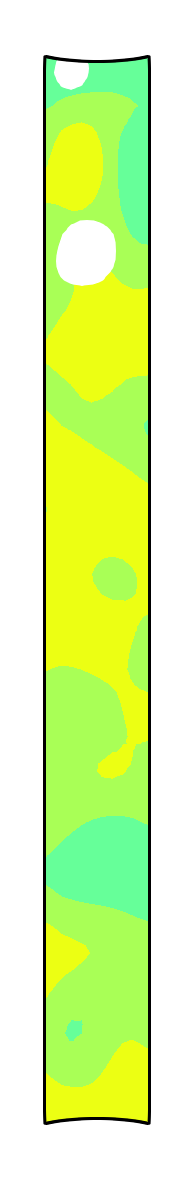
\includegraphics[width=\textwidth]{Chapter5/figures/spallation/gc_1}
  \end{subfigure}
  \begin{subfigure}{0.08\textwidth}
    \centering
    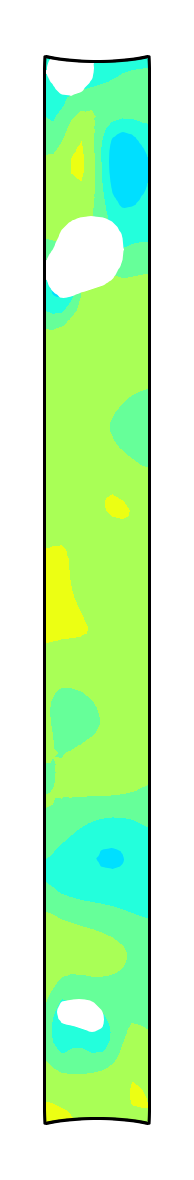
\includegraphics[width=\textwidth]{Chapter5/figures/spallation/gc_2}
  \end{subfigure}
  \begin{subfigure}{0.08\textwidth}
    \centering
    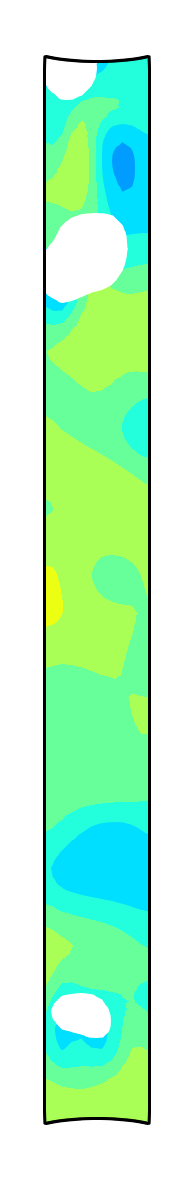
\includegraphics[width=\textwidth]{Chapter5/figures/spallation/gc_3}
  \end{subfigure}
  \begin{subfigure}{0.08\textwidth}
    \centering
    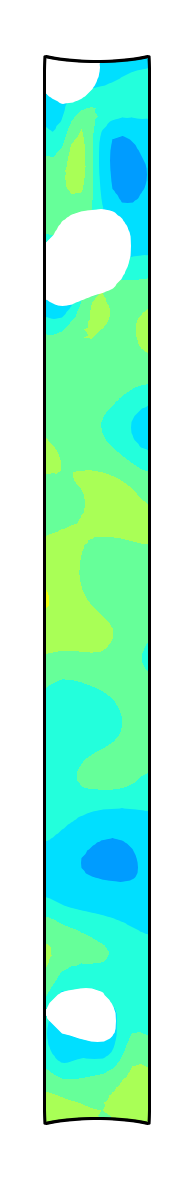
\includegraphics[width=\textwidth]{Chapter5/figures/spallation/gc_4}
  \end{subfigure}
  \begin{subfigure}{0.08\textwidth}
    \centering
    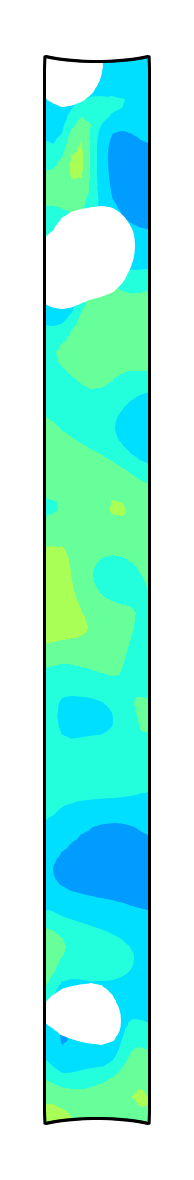
\includegraphics[width=\textwidth]{Chapter5/figures/spallation/gc_5}
  \end{subfigure}
  \begin{subfigure}{0.08\textwidth}
    \centering
    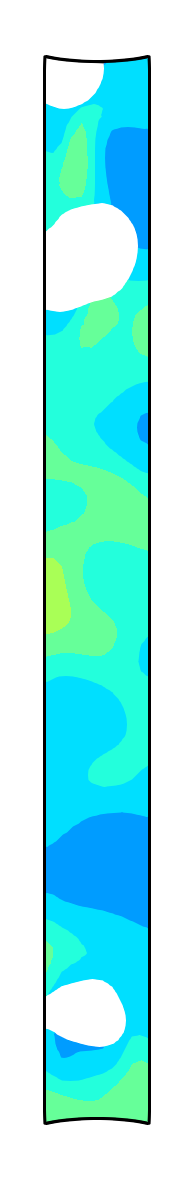
\includegraphics[width=\textwidth]{Chapter5/figures/spallation/gc_6}
  \end{subfigure}
  \begin{subfigure}{0.08\textwidth}
    \centering
    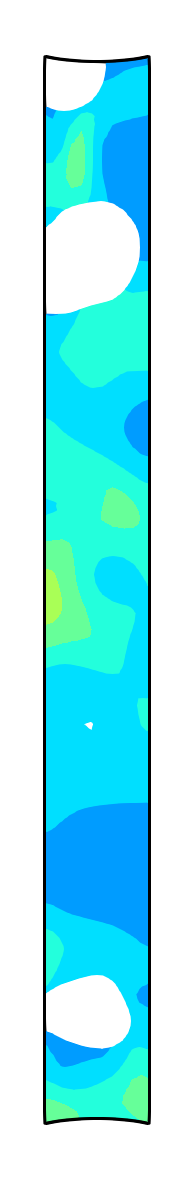
\includegraphics[width=\textwidth]{Chapter5/figures/spallation/gc_7}
  \end{subfigure}
  \begin{subfigure}{0.08\textwidth}
    \centering
    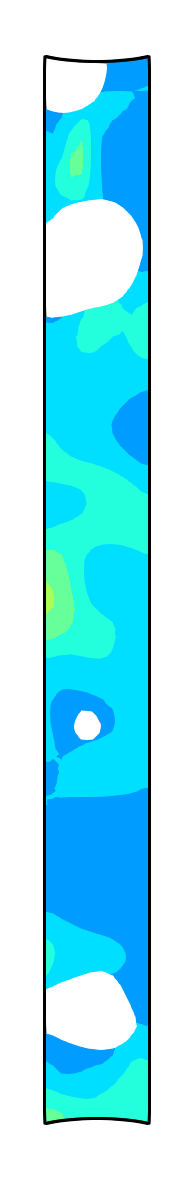
\includegraphics[width=\textwidth]{Chapter5/figures/spallation/gc_8}
  \end{subfigure}
  \begin{subfigure}{0.08\textwidth}
    \centering
    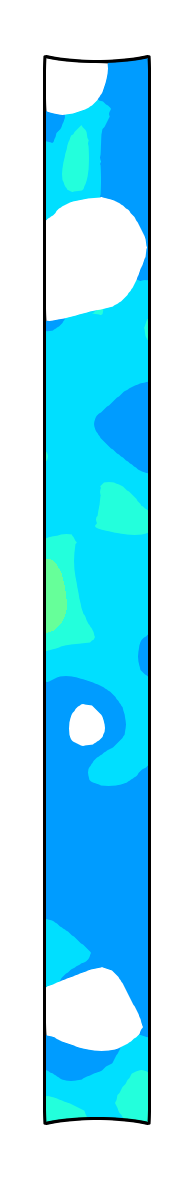
\includegraphics[width=\textwidth]{Chapter5/figures/spallation/gc_9}
  \end{subfigure}
  \begin{subfigure}{0.08\textwidth}
    \centering
    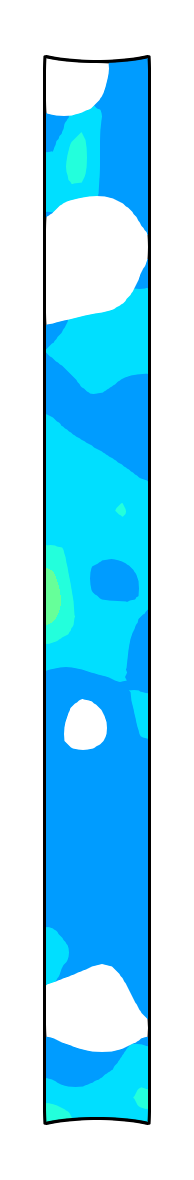
\includegraphics[width=\textwidth]{Chapter5/figures/spallation/gc_10}
  \end{subfigure}
  \begin{subfigure}{0.1\textwidth}
    \centering
    \caption*{$g_c$}
    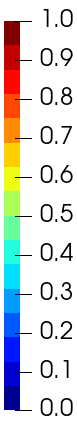
\includegraphics[width=0.7\textwidth]{Chapter5/figures/spallation/colorbar_gc}
  \end{subfigure}
  \caption{The coalescence degradation function right after each shut-down event. The region within the contour of $d \leqslant 0.75$ is removed to visualize in-plane fracture.}
  \label{fig: Chapter5/spallation/animation_gc}
\end{figure}
